\documentclass[12pt]{article}
\usepackage{amsmath}
\usepackage[lmargin = 1in, rmargin = 1in, tmargin = 1in, bmargin = 1in]{geometry}
\usepackage[none]{hyphenat}
\usepackage{graphicx}
\usepackage{subcaption}
\usepackage{float}

\title{\textbf{Problem 1(3)\\MATLAB lsqnonlin Implementation}}
\author{Aditya Vipradas\\ASU ID: 1209435588}
\begin{document}
\maketitle
Non-linear regression is performed on the given data to fit it to the given function using the \emph{lsqnonlin} function in MATLAB. The default stopping criterion of 1e-6 is used. Initial guess value is (1,1). The values of $A_{12}$ and $A_{21}$ obtained after the implementation are 1.9584 and 1.6892 respectively which agree with the gradient descent implementation with slight discrepancy. Levenberg-Marquardt algorithm is put to use. Refer the plot below that displays this curve fit. Also refer the attached code.
\begin{figure}[H]
\begin{center}
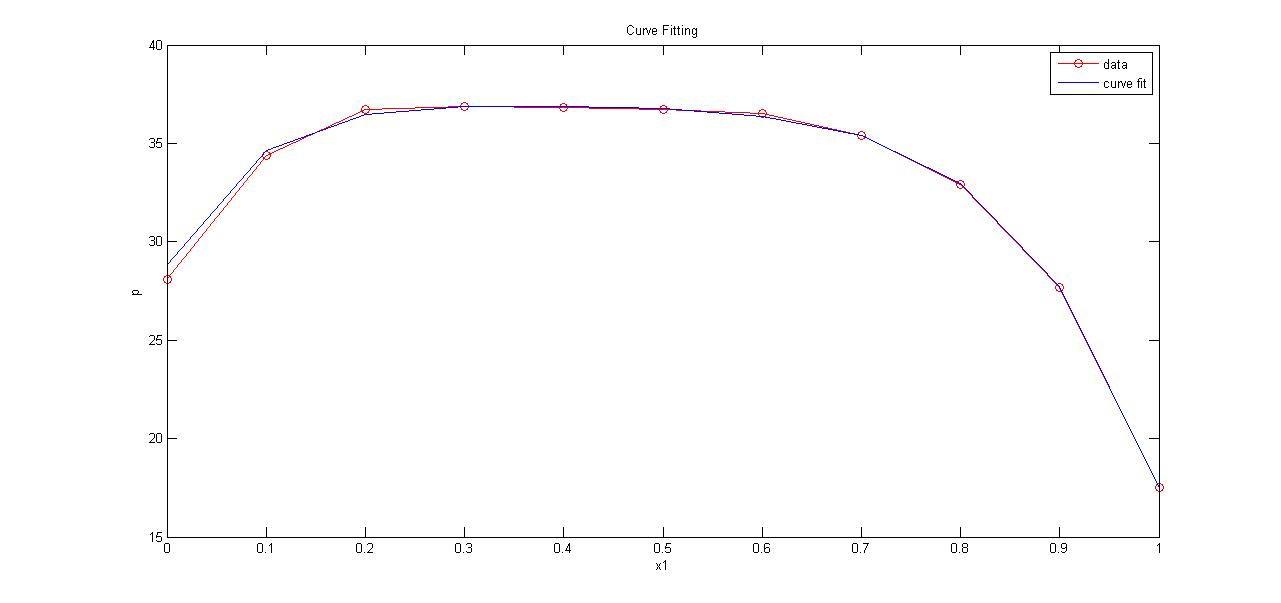
\includegraphics[scale=0.4]{curve.jpg}
\caption{Curve fit}  
\end{center}
\end{figure}
\end{document}